%\begin{figure}[ht]
%    \centering
%    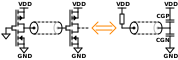
\includegraphics[width=0.50\textwidth]{3_modeling/figures/logicGatesModelMathieu.pdf}
%    \caption{Electrical equivalent model of two inverters interconnected with each other.}
%    \label{fig_equivLogicGateStdCell}
%\end{figure}

\begin{figure}[ht]
    \centering
    \begin{subfigure}{0.52\textwidth}
        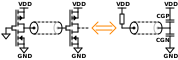
\includegraphics[width=\textwidth]{3_modeling/figures/logicGatesModelMathieu.pdf}
        \caption{Electrical equivalent model of two inverters interconnected with each other, with the first one outputting a logical ONE value.}
        \label{sfig_equivCMOS}
    \end{subfigure}
    \hfill
    \begin{subfigure}{0.44\textwidth}
        
\includegraphics[width=\textwidth]{3_modeling/figures/stdCellLayoutSimple.pdf}
        \caption{Simplified top view of a Standard-Cell with two power rail metal levels. In blue are the logic interconnections inside the Standard-Cell.}
        \label{sfig_simpleSCS}
    \end{subfigure}
    \caption{Equivalent logic gates models used in the SCS model (\ref{sfig_equivCMOS}), and a simplified top view of a Standard-Cell with its size (\ref{sfig_simpleSCS}).}
    \label{fig_equivLogicGateStdCell}
\end{figure}